\documentclass[a4paper, landscape]{article}

\usepackage[utf8]{inputenc}
\usepackage[DIV=12]{typearea}
\usepackage{microtype}
\usepackage{float}
\usepackage{mathtools, amssymb}
\usepackage{parskip}
\usepackage{subcaption}
\usepackage{graphicx}
\usepackage[colorlinks=true]{hyperref}

\title{8}
\date{} 

\graphicspath{ {../images} }

\hypersetup{linktoc=all}

\begin{document}
\maketitle
\section{Meta Image}
\ref{fig:bo}, \ref{fig:ko} show the original and the noisy images that are to be fed to  the bilateral filter.

As $\sigma$ increases, the noise in both images increases. 
Since, the resolution of the Kodak image is much higher than the Barbara image, the effect of noise on the details is lesser.
\begin{figure}
    \centering
    \begin{subfigure}{0.33\linewidth}
        \centering
        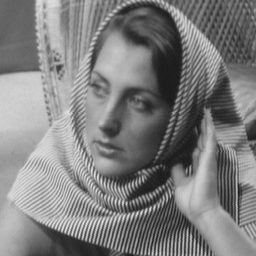
\includegraphics[width=\linewidth]{barbara256.png}
        \caption{Given image}
    \end{subfigure}
    \begin{subfigure}{0.33\linewidth}
        \centering
        \includegraphics[width=\linewidth]{barbara256,σ_noise5.png}
        \caption{Corrupted with Gaussian noise $\mu=0, \sigma=5$}
    \end{subfigure}
    \begin{subfigure}{0.33\linewidth}
        \centering
        \includegraphics[width=\linewidth]{barbara256,σ_noise10.png}
        \caption{Corrupted with Gaussian noise $\mu=0, \sigma=10$}
    \end{subfigure}
    \caption{Barbara image}
    \label{fig:bo}
\end{figure}
\begin{figure}
    \centering
    \begin{subfigure}{0.33\linewidth}
        \centering
        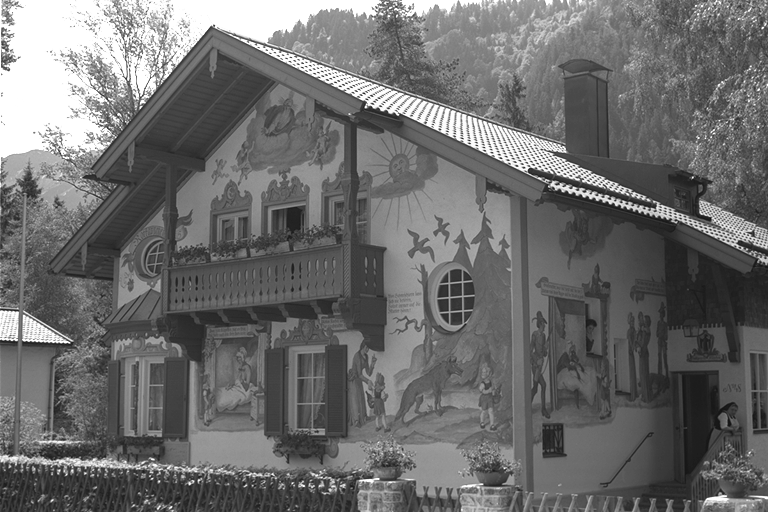
\includegraphics[width=\linewidth]{kodak24.png}
        \caption{Given image}
    \end{subfigure}
    \begin{subfigure}{0.33\linewidth}
        \centering
        \includegraphics[width=\linewidth]{kodak24,σ_noise5.png}
        \caption{Corrupted with Gaussian noise $\mu=0, \sigma=5$}
    \end{subfigure}
    \begin{subfigure}{0.33\linewidth}
        \centering
        \includegraphics[width=\linewidth]{kodak24,σ_noise10.png}
        \caption{Corrupted with Gaussian noise $\mu=0, \sigma=10$}
    \end{subfigure}
    \caption{Kodak image}
    \label{fig:ko}
\end{figure}
\section{Bilateral filter on original images}
\ref{fig:bs}, \ref{fig:ks} show the results of bilateral filter applied on the original Barbara and Kodak image.

As we go from left to right (increasing $\sigma_s, \sigma_r$), for both images, the image looks smoother but the textures get lost as is evident by focusing on the net in the background of the Barbara image, the text on the house in the Kodak image and the multi-layered window in the Kodak image. Also, some weird artifacts on the edges became more prominent like at the edges of facial features of Barbara.
\begin{figure}
    \centering
    \begin{subfigure}{0.33\linewidth}
        \centering
        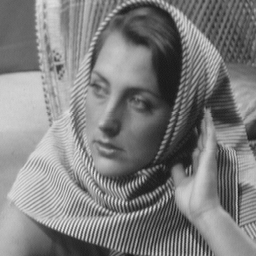
\includegraphics[width=\linewidth]{barbara256,σ_spatial0.1,σ_range0.1.png}
        \caption{$\sigma_s=0.1, \sigma_r=0.1$}
    \end{subfigure}
    \begin{subfigure}{0.33\linewidth}
        \centering
        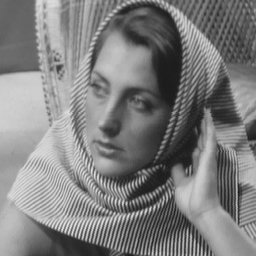
\includegraphics[width=\linewidth]{barbara256,σ_spatial2,σ_range2.png}
        \caption{$\sigma_s=2, \sigma_r=2$}
    \end{subfigure}
    \begin{subfigure}{0.33\linewidth}
        \centering
        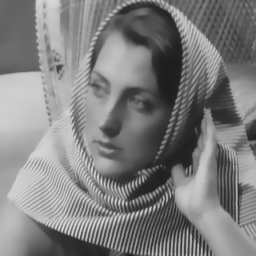
\includegraphics[width=\linewidth]{barbara256,σ_spatial3,σ_range15.png}
        \caption{$\sigma_s=3, \sigma_r=15$}
    \end{subfigure}
    \caption{Bilateral filter on original Barbara image}
    \label{fig:bs}
\end{figure}
\begin{figure}
    \centering
    \begin{subfigure}{0.33\linewidth}
        \centering
        
\includegraphics[width=\linewidth]{kodak24,σ_spatial0.1,σ_range0.1.png}
        \caption{$\sigma_s=0.1, \sigma_r=0.1$}
    \end{subfigure}
    \begin{subfigure}{0.33\linewidth}s
        \centering
        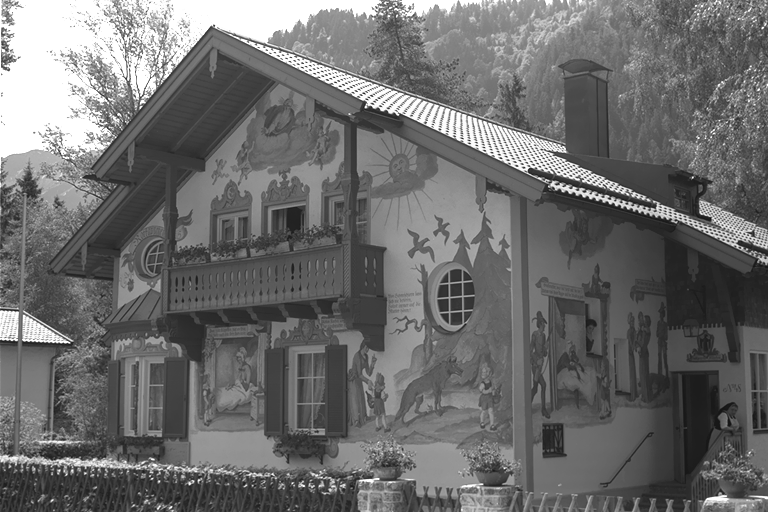
\includegraphics[width=\linewidth]{kodak24,σ_spatial2,σ_range2.png}
        \caption{$\sigma_s=2, \sigma_r=2$}
    \end{subfigure}
    \begin{subfigure}{0.33\linewidth}
        \centering
        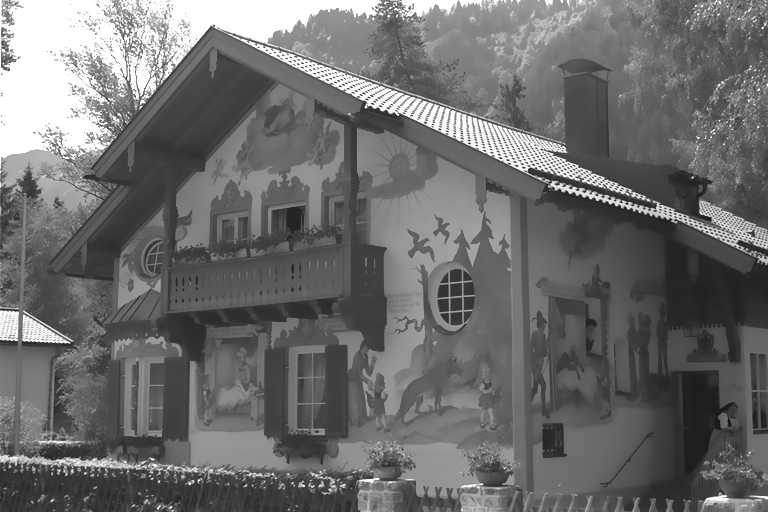
\includegraphics[width=\linewidth]{kodak24,σ_spatial3,σ_range15.png}
        \caption{$\sigma_s=3, \sigma_r=15$}
    \end{subfigure}
    \caption{Bilateral filter on original Kodak image}
    \label{fig:ks}
\end{figure}
\section{Bilateral filter on noisy images}
\ref{fig:bn}, \ref{fig:kn} show the results of bilateral filter applied on the noisy Barbara and Kodak image.

Bilateral filter of the biggest size $(\sigma_s=3, \sigma_r=15)$ does a good job in noise removal from both the images corrupted by both kind of Gaussian noise. 

Since, the resolution of the Kodak image is much higher than the Barbara image. The effect of noise on the details is lesser, hence its output doesn't look as bad as the output of Barbara image. 

As we go from left to right (increasing $\sigma_s, \sigma_r$), for both images, the image looks smoother but the textures get lost as evident by focusing at the net in the background of the Barbara image, the text on house in the Kodak image and the multi-layered window in  the Kodak image. Also, some weird artifacts on the edges become more prominent like at the edges of facial features of Barbara.
\begin{figure}
    \centering
    \begin{subfigure}{0.33\linewidth}
        \centering
        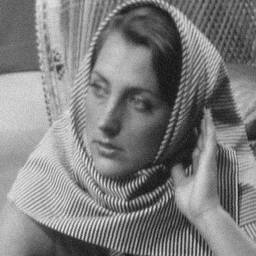
\includegraphics[width=\linewidth]{barbara256,σ_noise5,σ_spatial0.1,σ_range0.1.png}
        \caption{$\mu, \sigma = 0, 5, \sigma_s=0.1, \sigma_r=0.1$}
    \end{subfigure}
    \begin{subfigure}{0.33\linewidth}
        \centering
        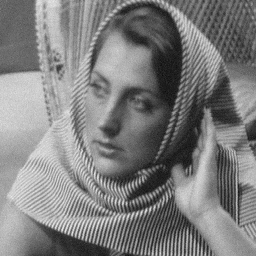
\includegraphics[width=\linewidth]{barbara256,σ_noise5,σ_spatial2,σ_range2.png}
        \caption{$\mu, \sigma = 0, 5, \sigma_s=2, \sigma_r=2$}
    \end{subfigure}
    \begin{subfigure}{0.33\linewidth}
        \centering
        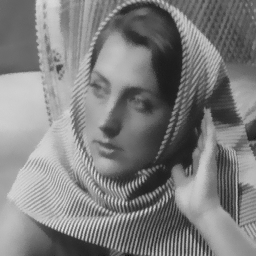
\includegraphics[width=\linewidth]{barbara256,σ_noise5,σ_spatial3,σ_range15.png}
        \caption{$\mu, \sigma = 0, 5, \sigma_s=3, \sigma_r=15$}
    \end{subfigure}
    \begin{subfigure}{0.33\linewidth}
        \centering
        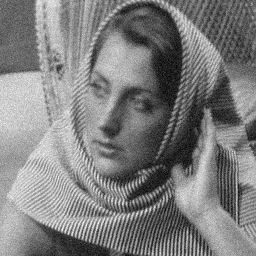
\includegraphics[width=\linewidth]{barbara256,σ_noise10,σ_spatial0.1,σ_range0.1.png}
        \caption{$\mu, \sigma = 0, 10, \sigma_s=0.1, \sigma_r=0.1$}
    \end{subfigure}
    \begin{subfigure}{0.33\linewidth}
        \centering
        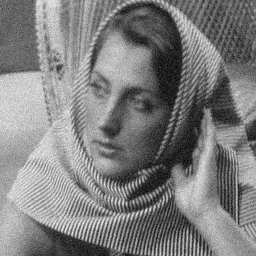
\includegraphics[width=\linewidth]{barbara256,σ_noise10,σ_spatial2,σ_range2.png}
        \caption{$\mu, \sigma = 0, 10, \sigma_s=2, \sigma_r=2$}
    \end{subfigure}
    \begin{subfigure}{0.33\linewidth}
        \centering
        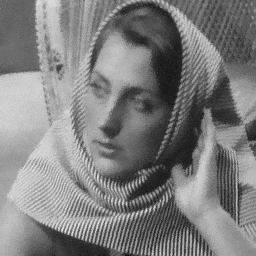
\includegraphics[width=\linewidth]{barbara256,σ_noise10,σ_spatial3,σ_range15.png}
        \caption{$\mu, \sigma = 0, 10, \sigma_s=3, \sigma_r=15$}
    \end{subfigure}
    \caption{Bilateral filter on noisy Barbara images}
    \label{fig:bn}
\end{figure}
\begin{figure}
    \centering
    \begin{subfigure}{0.33\linewidth}
        \centering
        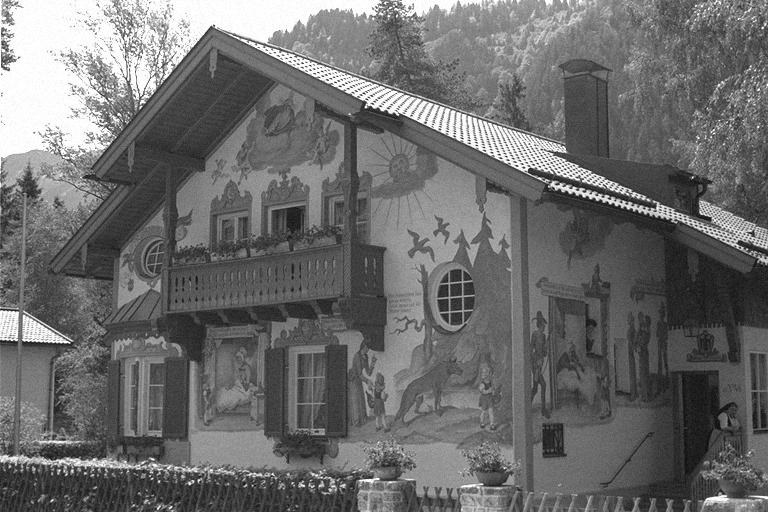
\includegraphics[width=\linewidth]{kodak24,σ_noise5,σ_spatial0.1,σ_range0.1.png}
        \caption{$\mu, \sigma = 0, 5, \sigma_s=0.1, \sigma_r=0.1$}
    \end{subfigure}
    \begin{subfigure}{0.33\linewidth}
        \centering
        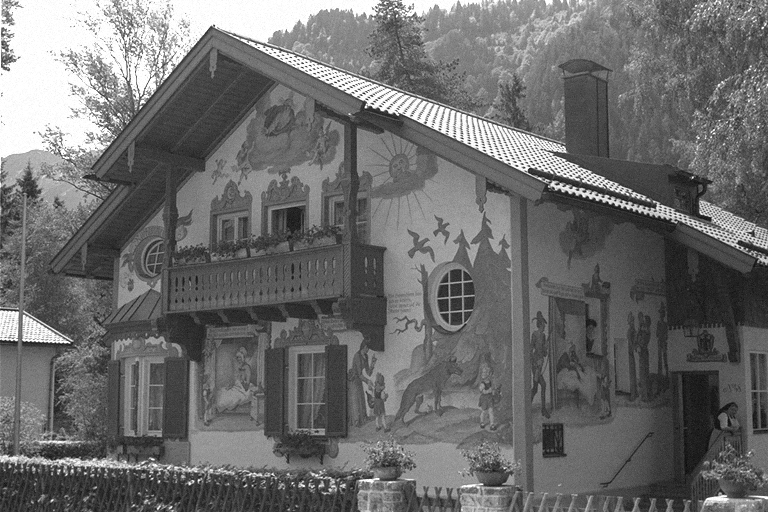
\includegraphics[width=\linewidth]{kodak24,σ_noise5,σ_spatial2,σ_range2.png}
        \caption{$\mu, \sigma = 0, 5, \sigma_s=2, \sigma_r=2$}
    \end{subfigure}
    \begin{subfigure}{0.33\linewidth}
        \centering
        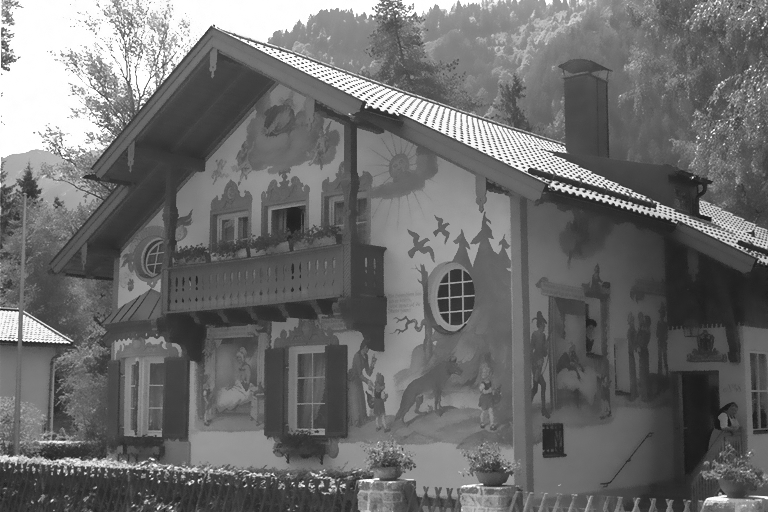
\includegraphics[width=\linewidth]{kodak24,σ_noise5,σ_spatial3,σ_range15.png}
        \caption{$\mu, \sigma = 0, 5, \sigma_s=3, \sigma_r=15$}
    \end{subfigure}
    \begin{subfigure}{0.33\linewidth}
        \centering
        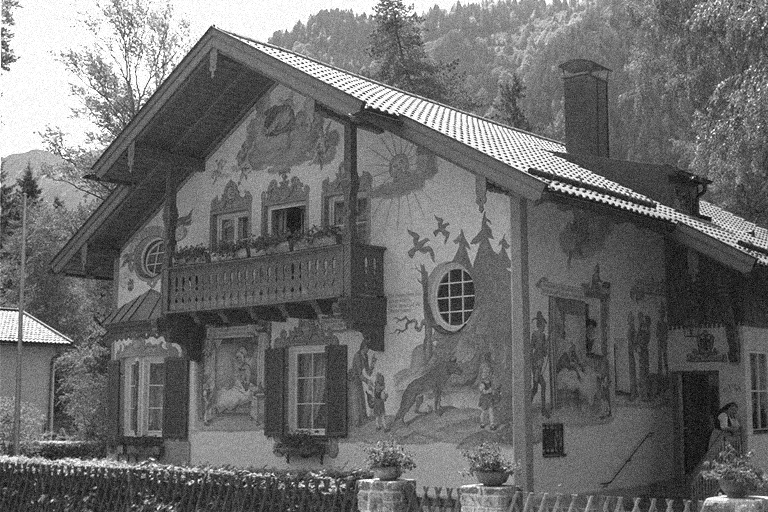
\includegraphics[width=\linewidth]{kodak24,σ_noise10,σ_spatial0.1,σ_range0.1.png}
        \caption{$\mu, \sigma = 0, 10, \sigma_s=0.1, \sigma_r=0.1$}
    \end{subfigure}
    \begin{subfigure}{0.33\linewidth}
        \centering
        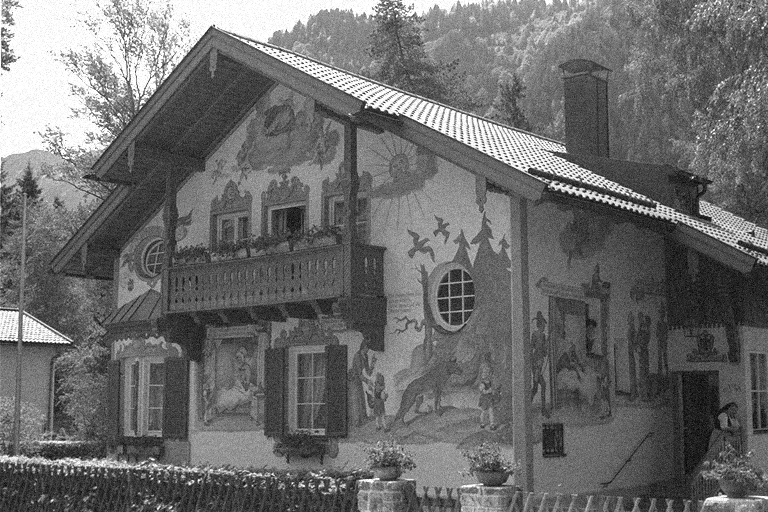
\includegraphics[width=\linewidth]{kodak24,σ_noise10,σ_spatial2,σ_range2.png}
        \caption{$\mu, \sigma = 0, 10, \sigma_s=2, \sigma_r=2$}
    \end{subfigure}
    \begin{subfigure}{0.33\linewidth}
        \centering
        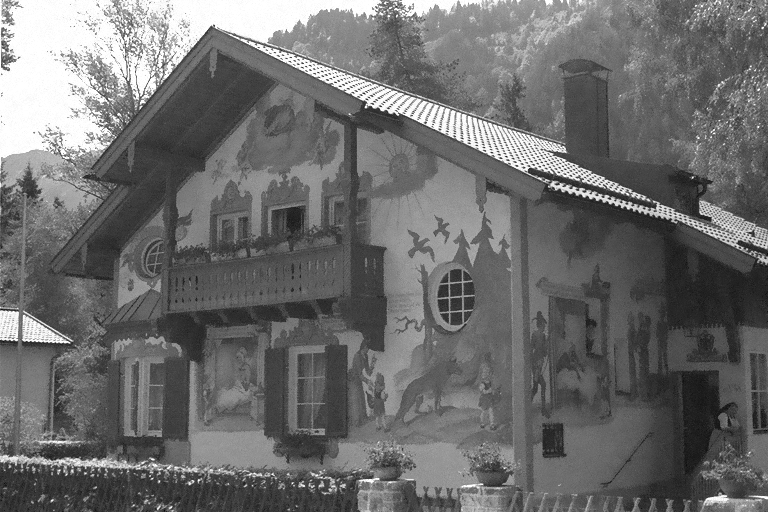
\includegraphics[width=\linewidth]{kodak24,σ_noise10,σ_spatial3,σ_range15.png}
        \caption{$\mu, \sigma = 0, 10, \sigma_s=3, \sigma_r=15$}
    \end{subfigure}
    \caption{Bilateral filter on noisy Kodak images}
    \label{fig:kn}
\end{figure}
% \section{Bilateral filter creation}

{\it Note the size of the filter is such that it includes the points at most ${\lceil3\sigma_s\rceil}$ away from the center point.
}
\end{document}